\documentclass[11pt, oneside]{article}   	% use "amsart" instead of "article" for AMSLaTeX format
\usepackage{geometry}                		% See geometry.pdf to learn the layout options. There are lots.
\geometry{letterpaper}                   		% ... or a4paper or a5paper or ... 

\usepackage[english]{babel}
\usepackage{url, verse}
\usepackage{pstricks, tikz}
\usepackage[T1]{fontenc}
\usepackage{setspace}
\usepackage{graphicx, wrapfig, capt-of}
\usepackage[normalem]{ulem} %for \sout
\usepackage{amssymb}
\usepackage{color}
\usepackage{tipa}
\usepackage{multicol, bold-extra, xcolor}
\raggedcolumns

\usepackage{stackengine}
\usepackage{array}
\newcolumntype{P}[1]{>{\centering\arraybackslash}p{#1}}
\newcolumntype{M}[1]{>{\centering\arraybackslash}m{#1}}
\usepackage{hhline,multirow, chngpage}
\newcommand*\rot{\rotatebox{90}}

\usepackage{linguex} %declare this package after tipa and graphicx
\renewcommand{\firstrefdash}{}
\usepackage{qtree}
%\usepackage{tree-dvips} %copy tree-dvips folder to make this work
\qtreecenterfalse

\newcommand{\cbox}[2]{{\color{#1}\fbox{\normalcolor#2}}} %colored text boxes

\usepackage{float}
\usepackage{tcolorbox, enumitem}
\usepackage{phonrule}

\usepackage{fancyhdr}
\pagestyle{fancy}{
\fancyhead[L]{Roberto Petrosino}
\fancyhead[C]{LING2010Q}
\fancyhead[R]{5: Syntax}
\renewcommand{\footrulewidth}{0pt}
\renewcommand{\headrulewidth}{0pt}}

\newenvironment{packed_enum}{
\begin{enumerate}
  \setlength{\itemsep}{1pt}
  \setlength{\parskip}{0pt}
  \setlength{\parsep}{0pt}
}{\end{enumerate}}

\newenvironment{packed_item}{
\begin{itemize}
  \setlength{\itemsep}{1pt}
  \setlength{\parskip}{0pt}
  \setlength{\parsep}{0pt}
}{\end{itemize}}

\renewcommand{\labelitemiii}{$\diamond$}


\title{{\normalsize LING 2010Q -- {\scshape Spring 2017}} \\ {\bfseries 5 - Syntax}}
\author{Roberto Petrosino \hspace{0.2cm} \url{roberto.petrosino@uconn.edu}}
\date{Oct 19 - Nov 1, 2017}

\begin{document}

\maketitle
\vspace{-1cm}
{\small \tableofcontents}

\newpage

\section{Basic concepts (back to week 1)}

\ex. Recall the basic questions of linguistic theory:
	\a. What exactly does a native speaker {\em know} about their language? $\leftarrow$
	\b. How is that knowledge acquired?
	\c. How is that knowledge put to use?
	\z.
In this class we focus mostly on the first question, but the other two are important as well.

\ex. A challenge in answering the first question is that speakers do not have direct access to the knowledge they have of their language. 

\subsection{Activity 1: Tacit knowledge.} 

{\itshape Consider the following sentences.}

\begin{enumerate}
\item John expected to surprise him.
\item I wonder who John expected to surprise him.
\item I wonder who John expected to surprise.
\end{enumerate}

\noindent{\itshape In each case, who is surprising whom?  Do you know what principles you use to decide this?  Did anyone teach you these?}

\ex. Many properties of language are {\bfseries recursive}, which means that they can be reiterated over and over again. For example:
\a. {[}Amanda]
\b. {[[}Amanda]'s boyfriend]
\c. {[[[}Amanda]'s boyfriend]'s sister]
\d. {[[[[}Amanda]'s boyfriend]'s sister]'s son]
\e. {[[[[[}Amanda]'s boyfriend]'s sister]'s son]'s toy] \hfill {\itshape ...etc}

\ex. Another example:
\a. {[}Dad bought a cat].
\b. {[}Rose said [(that) Dad bought a cat]].
\c. {[}Jon thinks [(that) Rose said [(that) Dad bought a cat]]].
\d. {[}Mark believes [(that) Jon thinks [(that) Rose said [(that) [Dad bought a cat]]]]].
\e. {[}Luke wonders [whether Mark believes [(that) Jon thinks [(that) Rose said [(that) Dad bought a cat]]]]].

\ex. {\bfseries Recursion} is theoretically {\bfseries unlimited}; however, our processing memory is limited, so our recursive abilities are limited.

\ex.??{[}The dog [the boy [the mom [the cat [...] scratched] scolded ] found ] ran away].

\ex. When we learn our first language, our {\em knowledge of that language} is:
	\a. {\bfseries tacit}, namely not explicit: we know things we don't know how we know
	\b. {\bfseries complex}: we can form pretty complicated sentences when we are pretty young
	\c. {\bfseries untaught}: nobody really {\em taught} us how to express ourselves in our first language
	\d. {\bfseries the poverty of stimulus}: at the age of 7 we typically become {\em native} in our language, despite impoverished and noisy evidence.
	\z.
{\itshape Why is that?} Noam Chomsky theorized that we are able to acquire languages because, as humans, we are equipped with a {\bfseries Universal Grammar} (UG). We can imagine UG as a blueprint of language communication, children refer to when acquiring a language; we all are endowed with it innately. Evidence for that mainly comes from the following:
	\a.	Acquisition is typically rapid and successful across children and across languages.
	\b.	Deep analysis reveals many similarities between superficially very different languages.
	\c.	Any human can learn any human language.

\section{Syntax}

\ex. syntax < Gr. {\itshape syn} `with' $+$ {\itshape taxis} `order'. \\ 
It refers to how discrete elements may combine into complex entities, according to a limited set of rules. 

\ex. The first thing that syntax does is {\bfseries categorizing}, i.e. dividing the basic building blocks of the combinations into different categories on the basis of shared properties. 

\begin{center}
\begin{tabular}{| c || c |}\hline
\multicolumn{2}{|c|}{\bfseries \scshape syntactic categories} \\ \hline
{\scshape lexical categories}	&	{\scshape functional categories} \\ \hline
nouns	&	articles (determiners) \\ 
adjectives	&	auxiliaries (be, have)  \\
verbs	&  modals (can, would, shoud, ...)\\
adverbs	&  particles (at, in, against, up, with, ...) \\
prepositions &	... \\ \hline
\end{tabular}
\end{center}

\ex. Let's revise syntactic categories one more time. There are a few tests you can use to identify each of those.
	\a. Nouns: the \underline{\hspace{1cm}}
	\b. Verbs: Mary will \underline{\hspace{1cm}}
	\c. Adjectives: the \underline{\hspace{1cm}} girl
	\d. Adverbs: Mary \underline{\hspace{1cm}} left
	\e. Prepositions: dance \underline{\hspace{1cm}} it

\ex. After categorizing, syntax needs to seek out how to arrange each of the categories in a coherent way. For example in English:
\ag. Bart ran. \\
N V \\
\bg. *Ran Bart. \\
V N \\ 
\cg. *Chased Bart John. \\
V N N \\
\dg. John gave Maggie Lisa. \\
N V N N \\

\ex. So, to wrap up:
	\a. Acceptable sentences of English:
		\a. N V
		\b. N V N
		\c. N V N N
		\z.
	\b. Unacceptable as sentences of English:
		\a. N N
		\b. V N
		\c. V N N

\subsection{Activity 2: Patterns and categories}
		
{\itshape State the categories found in sentences below and the patterns involved. Then give another sentence that fits that pattern using completely different words.}

\begin{enumerate}
\item John came home tired.
\item John heard Maggie clearly.
\item Lisa picked Maggie up.
\item Mary thinks Bart chased Lisa.
\end{enumerate}

\section{Syntactic rules and trees}

\ex. Let's play a bit. Read the following string of words aloud to yourself a couple of times.
	\a.[]
		\a.[a.] A enjoy delicious I cereal night of often at bowl.
		\z.
	\z.
{\em Done?} Now, cover up the paper and try to repeat it back out loud. How did it go? Try to do the same with the following string of words:
	\a.[]
		\a.[b.] I often enjoy a delicious bowl of cereal at night.
		

\ex. Cover it up and repeat \LLast[b] out loud --- better, right? Why do you think it was so much easier?

\begin{itemize}
\item If sentences were just words put together linearly, then we wouldn't have any feeling for meaningful subparts of sentences.
\item Every time we produce or understand a sentence, we are grouping words into phrases, and then {\itshape phrases} into bigger phrases (yes, that's recursion!)
\item Therefore, when we speak, we organize words and phrases in complex, hierarchical structures. Syntacticians aim at discovering those structures, and understand how they work, by coming up with {\itshape grammars}.
\end{itemize}

\ex. A grammar is a set of rules and principles that constitute a scientific theory about human linguistic knowledge. These are rewriting rules:
	\a. S $\rightarrow$ NP VP
	\b. S $\rightarrow$ NP VP NP
	\c. S $\rightarrow$ NP VP NP NP
	\z.
They mean: the symbol {\itshape S} (input) may be rewritten as the symbols following the arrow (ouput; in the example above and below, {\itshape NP} stands for Noun Phrase, {\itshape VP} for Verb Phrase). In case of multiple rewriting rules having the same input:
	\a. NP $\rightarrow$ John
	\b. NP $\rightarrow$ Lisa 
	\c. NP $\rightarrow$ Maggie
	\d. NP $\rightarrow$ Bart
	\z.
They may be abbreviated as: \\ 
	NP $\rightarrow$ John | Lisa | Maggie | Bart  

\ex. Computations for sentences in English begin with the \underline{initial symbol {\itshape S}}. \\
\vspace{-1.5em}
\begin{center}
\begin{tabular}{l l}
{\itshape `Bart ran'}	&	\\
Start: S 		&	S $\rightarrow$ NP VP	\\ 
Step 1: NP  VP	&	NP $\rightarrow$ Bart \\
Step 2: Bart VP	&	VP $\rightarrow$ ran \\		
Step 3: Bart ran	&	 \\
\end{tabular}
\end{center}

\ex. These are also called {\bfseries phrase structure rules} (PSR). Compare this rules with the rules that we have used in phonology; the latter were context-sensitive rules, the former are context free. 

\ex. A convenient way of representing the structure of a sentence is a tree diagram, or phrase marker.

\begin{figure}[H]
\centering
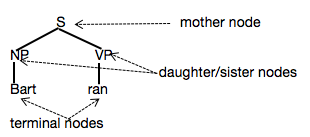
\includegraphics[scale=0.75]{tree.png}
\end{figure}

\ex. Trees and rules for {\itshape Bart chased Lisa}:

\begin{multicols}{2}

\Tree [.S [.NP {\itshape Bart} ] [.VP [.V {\itshape chased} ] [.NP {\itshape Lisa} ] ] ]

\columnbreak

\begin{itemize}
\item[] S $\rightarrow$ NP VP
\item[] NP $\rightarrow$ N 
\item[] N $\rightarrow$ Bart | Lisa
\item[] VP $\rightarrow$ V NP
\item[] V $\rightarrow$ chased
\end{itemize}

\end{multicols}

\subsection{Activity 3: Rewriting rules and tree diagrams}

{\itshape Write the syntactic rules and the corresponding tree diagrams for the following sentences. Remember that a sentence always starts with {\itshape S}.}

\begin{center}
\begin{tabular}{| P{0.4\textwidth} | P{0.4\textwidth} |}\hline
\multicolumn{2}{|c|}{a. Emma kicked the ball.}	\\ \hline
{\scshape Tree Diagram}	&	{\scshape Rules} \\
						&						   \\[5cm] \hline
\end{tabular}
\end{center}

\begin{center}
\begin{tabular}{| P{0.4\textwidth} | P{0.4\textwidth} |}\hline
\multicolumn{2}{|c|}{b. Christos ate the whole cake.}	\\ \hline
{\scshape Tree Diagram}	&	{\scshape Rules} \\
						&						   \\[5cm] \hline
\multicolumn{2}{|c|}{c. Steven wrote an article.}	\\ \hline
{\scshape Tree Diagram}	&	{\scshape Rules} \\
						&						   \\[5cm] \hline
\multicolumn{2}{|c|}{d. Claudia put the book on the desk.}	\\ \hline
{\scshape Tree Diagram}	&	{\scshape Rules} \\
						&						   \\[5cm] \hline
\end{tabular}
\end{center}

\begin{center}
\begin{tabular}{| P{0.4\textwidth} | P{0.4\textwidth} |}\hline
\multicolumn{2}{|c|}{e. Vanessa went to the Philippines.}	\\ \hline
						&						   \\[5cm] \hline
\end{tabular}
\end{center}

\section{Semantic Ambiguity}

\ex. A sentence is {\em semantically ambiguous} if it has more than one meaning. In some cases, the semantic ambiguity can be traced to a syntactic ambiguity.

\subsection{ Activity 4: Ambiguity} 

{\itshape For each of the following sentences, let's consider whether they can have one or more interpretations.}

\begin{enumerate}
\item Old men and women received the medication.
\item Michael hit the man with the halibut.
\end{enumerate}

\newpage

{\itshape Syntactic relations among constituents may help disambiguate the meaning. Let's try this out together.}

\begin{center}
\begin{tabular}{| P{0.4\textwidth} | P{0.4\textwidth} |}\hline
\multicolumn{2}{|c|}{a. Michael hit [the man with halibut]}	\\ \hline
{\scshape Tree Diagram}	&	{\scshape Rules} \\
						&						   \\[5cm] \hline
Interpretation: \underline{\hspace{2.5cm}} & Interpretation: \underline{\hspace{2.5cm}}\\ \hline
\end{tabular}
\end{center}

\begin{center}
\begin{tabular}{| P{0.4\textwidth} | P{0.4\textwidth} |}\hline
\multicolumn{2}{|c|}{b. Michael [hit [the man] with halibut]} \\ \hline
{\scshape Tree Diagram}	&	{\scshape Rules} \\
						&						   \\[5cm] \hline
Interpretation: \underline{\hspace{2.5cm}} & Interpretation: \underline{\hspace{2.5cm}}\\ \hline
\end{tabular}
\end{center}

\section{Studying grammars}

\ex. Syntacticians aim at proposing grammars to account for observations made about a given language and test the predictions made by these grammars.

\ex. Syntacticians collect data from native speakers, by asking them {\bfseries judgments} about the well-formedness of sentences of their language.

\ex. Judging grammaticality is not simple: naïve native speakers give judgments of acceptability, which may be based on comprehensibility, notions of social correctness, ease of processing, etc. Syntacticians need to take care to decide which judgments reflect intuitions of (un-)grammaticality. Consider the following examples:
	\a. Colorless green ideas sleep furiously.
	\b. Colorless sleep furiously ideas green.
	\z.
What kind of observation can we make here? \\
{\em Your answer:}
\vspace{1cm}
	
\ex. In evaluating a grammar, we must see if the grammar predicts judgments of the speakers whose grammatical knowledge we are trying to account for.  This includes {\em both} judgments of grammaticality and ungrammaticality.
	\a. John ate.
	\b. *Ate John.
	\z.
It is not enough for a grammar to generate a), and it must not generate the ungrammatical sentence b).
	
\ex. Typically a grammar constructed for a small set of data will generate sentences beyond those the initial small set of data.  These are {\bfseries predictions} of the grammar.

\ex. If grammar G generates sentence S, G predicts that S is {\em grammatical}.

\ex. If grammar G doesn't generate sentence S, G predicts that S is {\em ungrammatical}.

\ex. If a grammar predicts that a grammatical sentence is ungrammatical, then the grammar {\bfseries undergenerates}. If a grammar predicts that an ungrammatical sentence is ungrammatical, then the grammar {\bfseries overgenerates}.

\ex. The ideal grammar of a language must have the following properties:
	\a.	full coverage of the facts: the more facts explained the better.
	\b.	simplicity: the simpler the theory --- fewer rules and symbols --- the better.
	\c.	fertility: a good theory makes testable predictions.
	\d.	depth of understanding: a good theory tells us why.

\section{Constituency}

\ex. What is a {\bfseries constituent?} Intuitively, it is a string of words that we can manipulate (i.e., move around, replace, delete, ?) a single chunk. 

\ex. We can make use of several {\bfseries constituency tests}, to identify syntactic constituents. They're pretty intuitive, but it is crucial how to perform them. The reasoning behind all of them is always the same: if a a string of words meaningfully passes most of them, that string of words can be deemed as a coherent syntactic unit.

\ex. {\bfseries \scshape Conjunction Test}. If a string of words can be conjoined, then they are a constituent.
	\a. Bill talked [to Mary]. 
		\a.[] We want to find out whether [to Mary] is a constituent. To do that, we can conjoined that phrase with a similar one, e.g.:
			\a.[a'] Bill talked [to Mary] {\em and} [to John].
			\z.
		\z.
	\b. Another example: John talked to Mary [on Friday].
		\a.[b'] John talked to Mary [on Friday] {\em and} [on Monday].

\ex. {\bfseries \scshape Proform Replacement Test}. If a string of words can be replaced by a proform, they form a constituent.
	\a. John saw [the cop]. 
	\b.[a'.] Mary talked to {\em him} (i.e., the cop). \\
	\c.[b.] Bill arrived [on Tuesday]. 
	\d.[b'.] Sen also arrived {\em then}. \\
	\e.[c.] Lisa [criticized Alex on Monday].
	\f.[c'.] Lisa [criticized Alex on Monday] and Kate {\em did so too}. 

\ex. {\bfseries \scshape Ellipsis Test}. If a string of words can be elided (i.e., left unpronounced), then they form a constituent.
	\a. Adam will [buy a donut] 
	\b.[a'.] Adam will [buy a donut] and Bill won't \sout{buy a donut}. \\
	\c.[b.] Mary took two [pictures of Greg].
	\d.[b'.] Mary took two [pictures of Greg] and Bill took four \sout{pictures of Greg}.

\ex. {\bfseries \scshape Dislocation Test}. If a string of words can be dislocated, then it is a constituent.
	\a. John will [read a book]. 
	\b.[a'.] {\em Read the book}, John will. \\
	\c.[b.] Mary loves [cats]. 
	\d.[b'.] {\em Cats}, Mary loves.

%\section{Relations between tree nodes}
%
%\ex. There are relations between tree nodes that are relevant to the statement of grammatical principles.  Three relations in particular are important.
%
%\ex. {\bfseries Dominance} \\
%Node A dominates node B when you can trace path downward along the branches of the tree from A to B.
%
%\begin{multicols}{2}
%
%\ex. \Tree [.A [.B D ] [.C [.E ] [.F ] ] ]
%
%\vfill
%\columnbreak
%
%\noindent A dominates B, C, D, E and F. \\
%C dominates E and F. \\
%C does {\em not} dominate A, B or D.
%
%\end{multicols}
%
%\ex. {\bfseries Precedence} \\
%If two nodes A and B are sisters and A is to the left of B, then A precedes B.
%	\a. {\em Corollary:} If A precedes B, then A and everything A dominates, precede B and everything B dominates. \\
%In the tree \LLast: B precedes C, E and F; D precedes C, E and F; E precedes F.
%
%\ex. {\bfseries C(onstituent)-command} \\
%A node X {\em c-commands} a node Y iff X nor Y dominates the other, and the first branching node dominating X also dominates Y.
%	\a. {\em Rule of thumb I}. \\ 
%``Any node that is contained in my sister, I c-command it.''
%	\b. {\em Rule of the thumb II}. \\
%Imagine every node of a tree as train stops. The train goes one node up and one node down; the stop (=node) at which the train stops is the {\em c-command domain} of the node the train has departed from.
%\vspace{-1em}
%\begin{figure}[H]
%\centering 
%\includegraphics[scale=0.75]{ccommand.png}
%\end{figure}
%
%\ex.[] Let's consider the figure above again. The train departs from B goes up one node and down another node, and stops at C; C is the c-command domain of node B.
%	\a. What about F? \underline{\hspace{3cm}}
%	\b. What about C? \underline{\hspace{3cm}}
%	\c. What about D? \underline{\hspace{3cm}}
%	
%\newpage
%
%\subsection{Activity 5: Nodal relations.}
%
%{\itshape Consider the following tree diagram and define the relations of dominance, precedence and c-command among nodes.}
%\begin{center}
%
%\Tree [.A [.B. [.D H I ] E ] [.C [.F L ] [.G M N ] ] ]
%
%\vspace{1em}
%
%\begin{tabular}{l l l l}
%Nodes B dominates:	& \underline{\hspace{1cm}}	&	Nodes D c-commands: &	\underline{\hspace{1cm}} \\
%Nodes G precedes:	& \underline{\hspace{1cm}}	&	Nodes D dominates:	& \underline{\hspace{1cm}} \\
%Nodes M c-commands:	& \underline{\hspace{1cm}}	&	Nodes D precedes: 	& \underline{\hspace{1cm}} \\
%Nodes E dominates:	& \underline{\hspace{1cm}}	&	Nodes F precedes: 	& \underline{\hspace{1cm}} \\
%Nodes C precedes: 	& \underline{\hspace{1cm}}	&	Nodes F c-commands:	& \underline{\hspace{1cm}} \\
%Nodes L c-commands:	& \underline{\hspace{1cm}}	&	Nodes F dominates: 	& \underline{\hspace{1cm}} \\
%\end{tabular}
%\end{center}
%
%\subsection{Activity 6: C-command at work}
%
%{\itshape Consider the two datasets below. How can we account for the distribution of {\normalfont himself} below?}
%
%\ex. \a. John saw himself.
%\b. John revealed himself to Mary.
%\c. Mary revealed John to himself.
%\d. John bought a picture of himself.
%\e. John gave an award to himself.
%
%\ex. \a. *Himself saw John.
%\b. *Himself revealed John to Mary.
%\c. *Mary revealed himself to John.
%\d. *Mary gave a picture of himself to John.
%\e. *A picture of John fell on himself.

\newpage

\section{Recap}

\ex. We don't have a direct access to how we correctly speak a language ? we just know we have learnt ({\bfseries tacit knowledge}) it when we were kids, without being explicitly taught. This led Chomsky to argue that we are endowed with a {\em Universal Grammar}, a set of principles children use to acquire the language(s) they are being exposed to.

\ex. {\bfseries Syntax} aims at catching how words are coherently organized in phrases, i.e. syntactic chunks. Phrases can be grouped together in order to form bigger phrases, such as sentences.

\ex. Syntax deals with organizing an incredible amount of words in a coherent way. However, it doesn't particularly care about the exact words, rather the {\bfseries syntactic category} each of them belongs to. By looking at how syntax of a language merges words, we can come up with patterns a given language always sticks to.

\ex. A {\bfseries grammar} is the set of rules a language uses to forms phrases. Syntacticians aim at explaining data collected from native speakers through {\em acceptability judgments}. A grammar is good, if it makes correct {\em predictions} about what is grammatical and what is not for a native speaker. 

\ex. {\em Phrases} can be represented in {\bfseries tree diagrams}; we can identify phrases by using {\bfseries constituency tests}.

%\ex. Tree diagrams are useful tools able to account for relations across nodes. The main nodal relations are: {\bfseries dominance, precedence and c-command}.

\end{document}